\section{Tests préliminaires}
Le but des tests préliminaires est de vérifier que les analyses effectuées dans la phase de recherche sont applicables et si la mise en
place du système imaginé lors de la phase de sélection du matériel est aussi efficace qu'espéré.

Il a été décidé de contrôler la télécommande via un système de préhenseur d'aimant de levage. Les données disponibles de la télécommande
ne stipule pas la force nécessaire à l'activation d'un de ses boutons, plusieurs préhenseurs sélectionné dans le stock du \Gls{fablab}
sont utilisés pour définir la force nécessaire à l'activation des touches.

\begin{itemize}
    \item Préhenseur 6VDC 4W, 0.4N -> 2N.
    \item Préhenseur 12VDC 7W, 0.6N -> 11N.
\end{itemize}

Les préhenseurs ont été installés sur une pièce imprimée en 3D permettant d'actionner la télécommande sans avoir des effets de reculs.
La hauteur est determinée de manière à pouvoir glisser la télécommande entre les plauqes tout en garantissant que la tige puisse se déployer sur
une longueur suffisante pour atteindre son pic de force.

\begin{figure}[H]
    \centering
    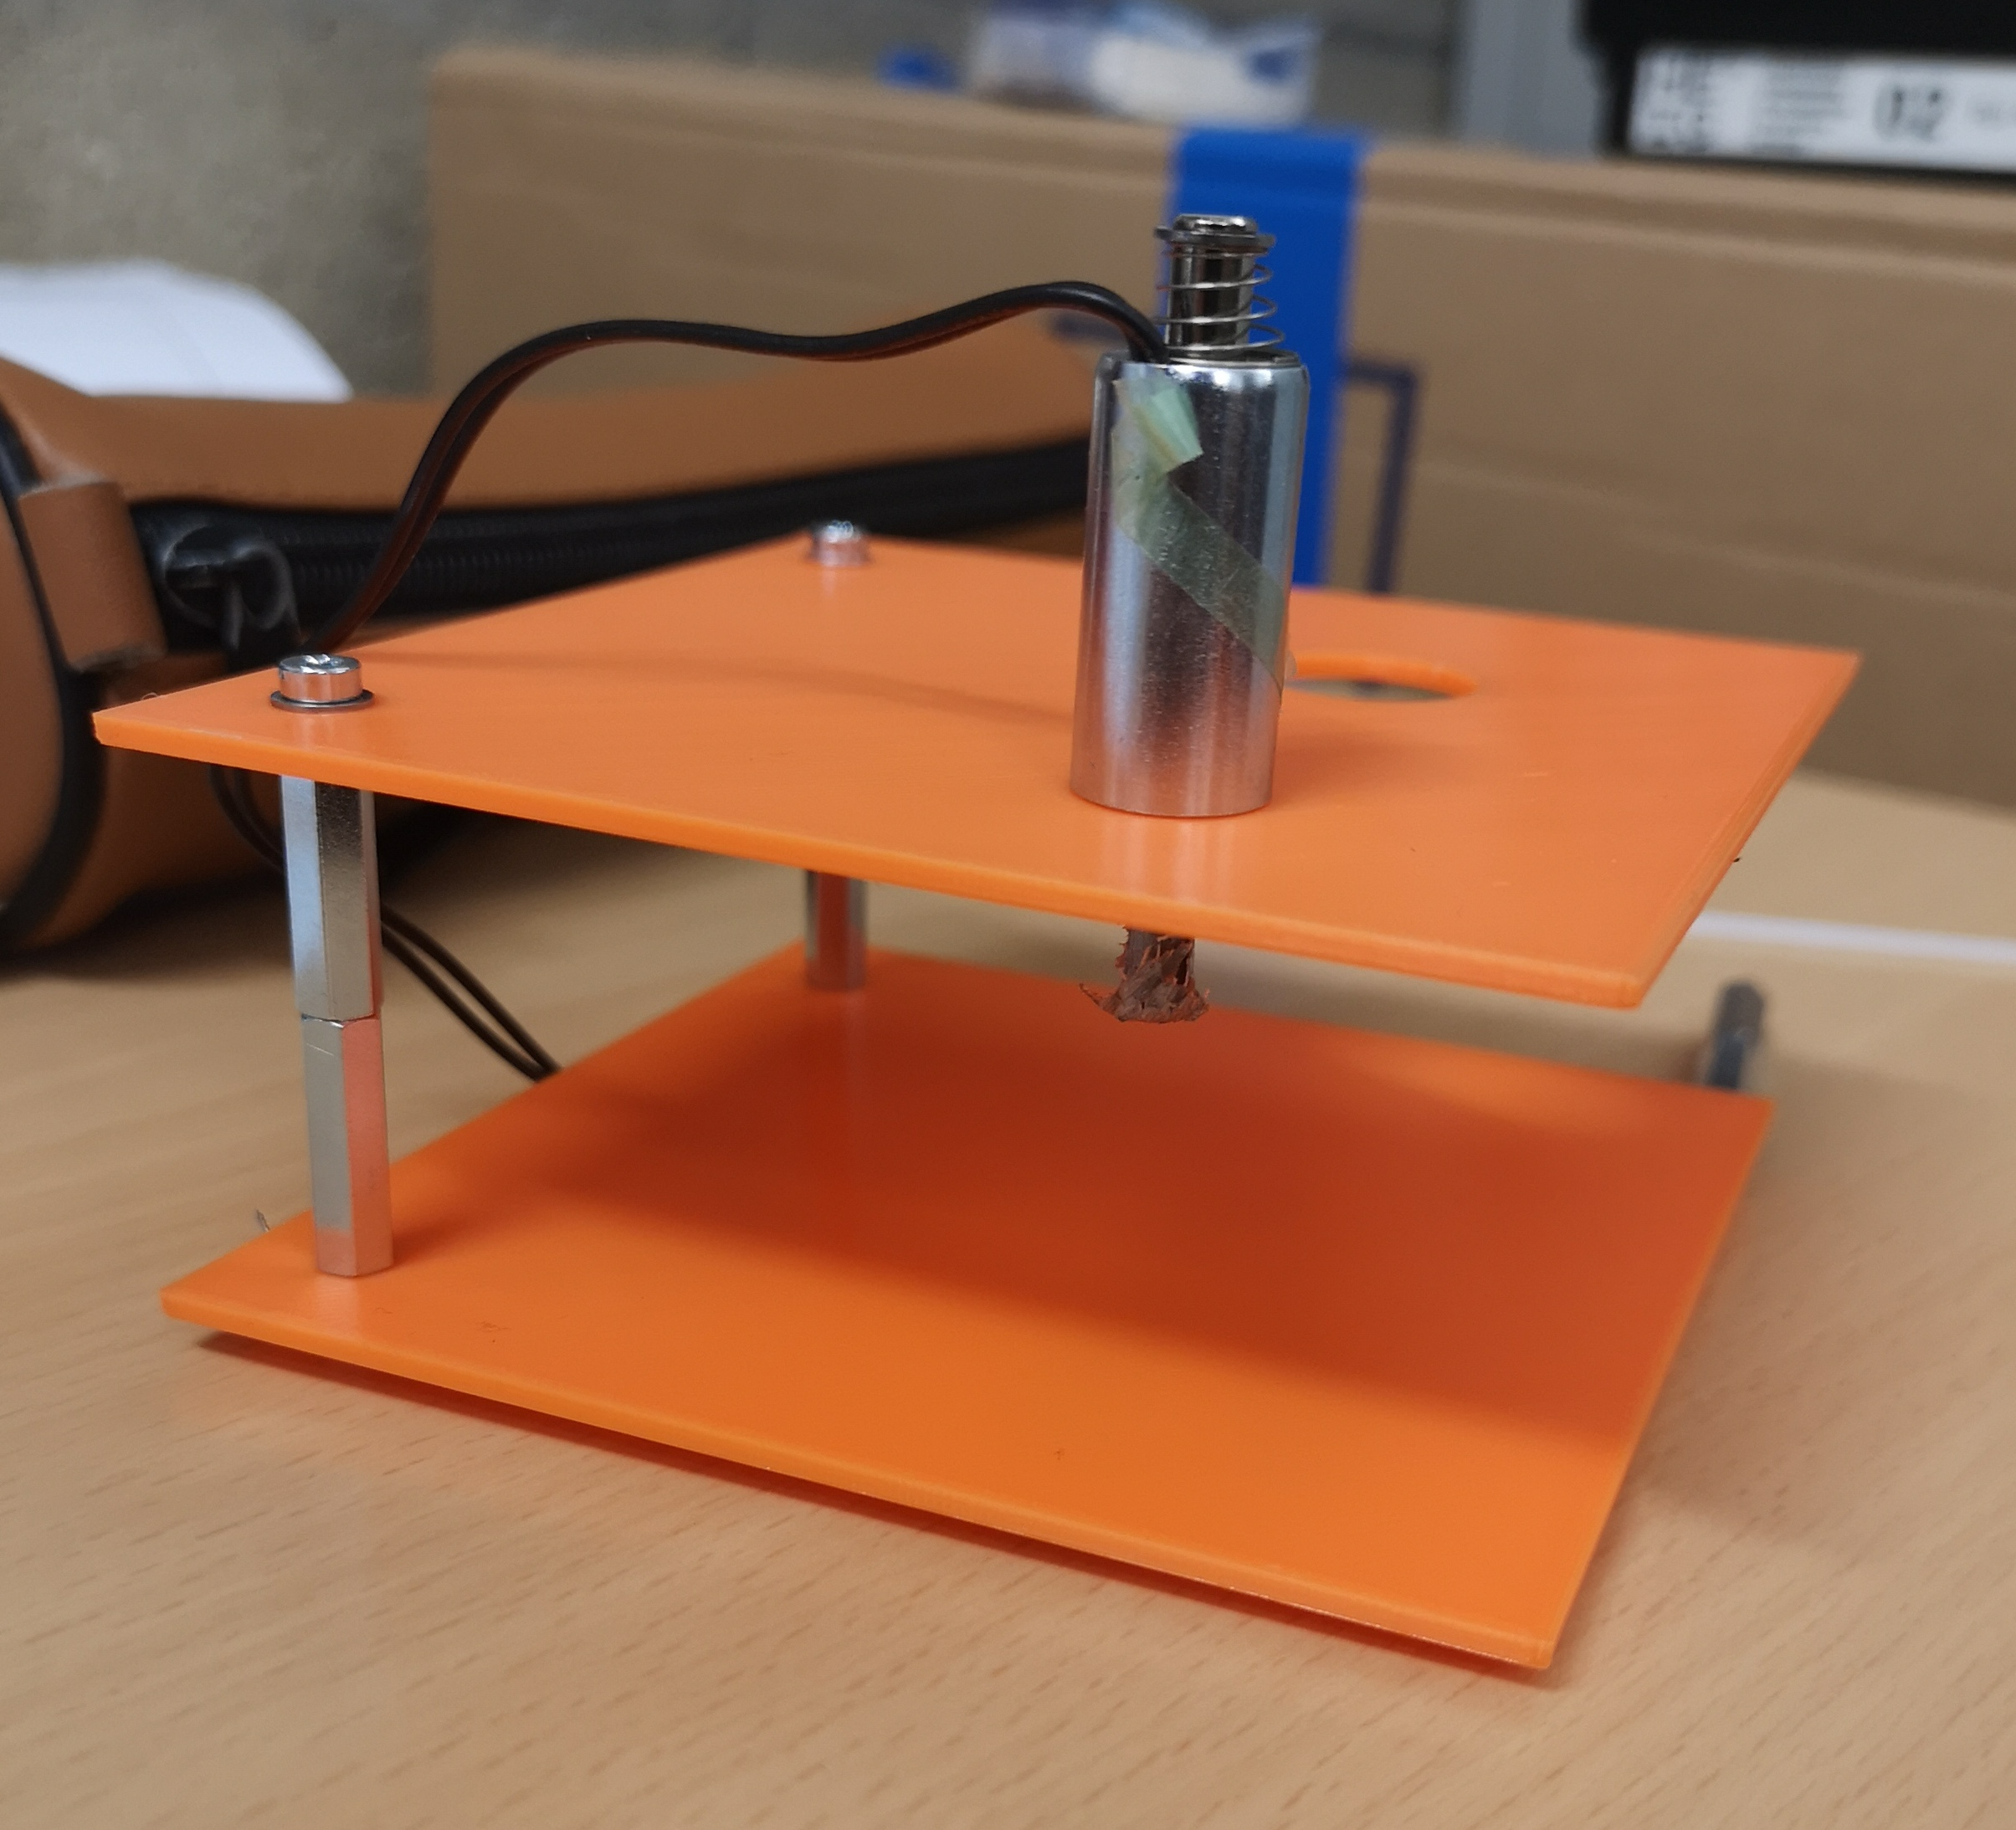
\includegraphics[width=10cm]{assets/figures/support_test_prehenseur.jpg}
    \caption{Système de préhension - Support de test}
\end{figure}

\begin{table}[h]
    \begin{center}
        \caption{Résultats du test de préhension}
        \begin{tabular}{|c|l|}
            Elements       & Boutons \\ \hline
            Préhenseur 2N  & OUI-NON \\
            Préhenseur 11N & OUI-NON \\
        \end{tabular}
    \end{center}
\end{table}\\

\section{Supports}

\subsection{Support pour jeu de préhenseur magnétique}
\subsection{Support de la télécommande}

\section{Programme}
\subsection{Pilotage des vérins}
\subsection{Communication}